\chapter{Projeto - Parte 1} \label{ch:projeto-parte1}

Esta parte do projeto incidiu principalmente sobre desenvolvimento de uma biblioteca, em Java, para providenciar abstrações dos subsistemas que representam conceito gerais de Inteligência Artificial (e.g., agente, ambiente) e outros conceitos relacionados (e.g., máquina de estados).

Para tal, foi necessário definir uma arquitetura de software que permitisse a implementação dos diferentes subsistemas de forma independente e modular, seguindo as diretrizes (i.e., métricas (ver secção~\ref{subsec:metricas}) e princípios (ver secção~\ref{subsec:principios})) que garantem a qualidade da arquitetura.

A implementação da biblioteca foi feita com base na consulta e compressão de diagramas UML e de sequência de forma a garantir a correta implementação dos diferentes subsistemas.

Por fim foi desenvolvido um jogo (ver secção~\ref{sec:desenvolvimento-do-jogo}) que integra a biblioteca desenvolvida, permitindo a interação com o jogador por meio de comandos em texto.


\section{Arquitetura de software}\label{sec:arquitetura-de-software}

A arquitetura de software aborda a complexidade inerente ao desenvolvimento de software por meio de uma série de vertentes que estão interligadas.

\subsection{Métricas}\label{subsec:metricas}

As métricas são medidas de quantificação da arquitectura de um software indicadoras da qualidade dessa arquitectura;

O acomplamento é uma métrica inter-modular que mede o grau de interdependência entre os módulos de um sistema. Pode ser medido através da:
\begin{itemize}
    \item \textbf{Direção}: Unidirecional vs Bidirecional (uni representa menos acoplamento);
    \item \textbf{Visibilidade}: Quando menor for a visibilidade de um módulo, menor é o seu acoplamento;
    \item \textbf{Ordem}: (de menos acoplamento para mais) Herança $\rightarrow$ Composição $\rightarrow$ Agregação $\rightarrow$ Associação $\rightarrow$ Dependência.
\end{itemize}

A coesão é uma métrica intra-modular que determina o nível de coerência funcional de um subsistema/módulo, seja pela sua organização (i.e., cada modulo está organizado por conteúdo) ou pela sua funcionalidade (e.g., \ti{single responsibility principle} - cada modulo tem uma única responsabilidade).

\subsection{Princípios}\label{subsec:principios}

Os princípios no contexto da arquitectura de software são um conjunto de convenções que orientam a sua definição, garantindo a qualidade de produção da mesma. Alguns exemplos são:
\begin{itemize}
    \item \textbf{Abstração}: Define a forma como os componentes de um sistema são representados, permitindo a ocultação de detalhes de implementação;
    \item \textbf{Modularização}: Ao qual está associado a decomposição (e.g, divisão do sistema em sub-módulos) e o encapsulamento (i.e., ocultação de detalhes de implementação e/ou manutenção de estado privado e interno);
    \item \textbf{Factorização}: Onde a arquitectura é dividida em camadas, cada uma com um conjunto de responsabilidades bem definidas. Pode ser estrutural (e.g, Herança) e Funcional (e.g, Delegação);
\end{itemize}


\section{Processo de Desenvolvimento de Software}\label{sec:processo-de-desenvolvimento-de-software}

O processo de desenvolvimento de software consiste na
criação da organização de um sistema de forma
progressiva, através de diferentes níveis de abstracção:

\begin{itemize}
    \item \textbf{Modelo (Conceptual)}: Representação abstrata do sistema, que define o que o sistema deve fazer, sem especificar como;
    \item \textbf{Arquitetura (Modelo Concreto)}: Representação concreta do sistema, que define como o sistema deve ser implementado;
    \item \textbf{Implementação}: Código fonte que implementa o sistema definindo como o sistema deve ser executado.
\end{itemize}

Consiste num processo iterativo, em que as diferentes actividades de desenvolvimento são alternadas ao longo do tempo em função do conhecimento e do nível de detalhe
envolvido. Essa alternância poderá ser circular (i.e., implementação $\rightarrow$ arquitectura $\rightarrow$ modelo $\rightarrow$ implementação).

\subsection{Tipos de Implementação}\label{subsec:tipos-de-implementacao}

\begin{table}[H]
    \centering
    \caption{Tipos de Implementação}
    \label{tab:tipos-de-implementacao}
    \vspace{0.2cm}
    \begin{tabular}{|l|l|p{8cm}|}
        \hline
        \textbf{Tipo}  & \textbf{Modelo Associado}  & \textbf{Designação}                                                                                        \\ \hline
        Estrutural     & \ti{UML}                   & Define a estrutura de um sistema, ou seja, a forma como os componentes se relacionam entre si.             \\ \hline
        Comportamental & \ti{Diagrama de Sequência} & Define o comportamento de um sistema, ou seja, a forma como os componentes interagem e comunicam entre si. \\ \hline
    \end{tabular}
\end{table}

Mais detalhadamente, os diagramas de sequência ou atividade representam o fluxo de controlo de um sistema, ou seja, a sequência de atividades que um sistema executa e a sua ordem. Definem-se como modelos de interação com uma organização bidirecional (i.e., horizontal $\rightarrow$ tempo e vertical $\rightarrow$ estrutura) e são compostos por diferentes elementos de modelação (e.g., mensagens, operadores, linha de vida).

Já a linguagem de modelação unificada (i.e., UML - \ti{Unified Modeling Language}) representa um modelo de comportamento com interação como perspetiva principal de modelação.
Este tipo de modelação descreve a forma como as partes de um sistema interagem entre si e com o exterior para produzir o comportamento do sistema.
No contexto do projeto, esta linguagem também ajudou a compreender os conceitos fundamentais associados a um sistema computacional (ver secção~\ref{sec:modelacao-de-um-sistema-computacional}) através da representação de diagramas de transição de estado.


\section{Modelação de um Sistema Computacional}\label{sec:modelacao-de-um-sistema-computacional}

Um sistema computacional geral, pode ser caracterizado de forma abstrata (ver figura~\ref{fig:sistema-computacional-abstrato}), através de uma representação de estado, que define em cada momento a configuração interna do
sistema, e de uma função de transformação que gera as saídas e o próximo estado em
função das entradas e do estado actual do sistema~\cite{isel:iasa:slides:intro-eng-soft-parte-3}.

\begin{figure}[H]
    \begin{center}
        \resizebox{100mm}{!}{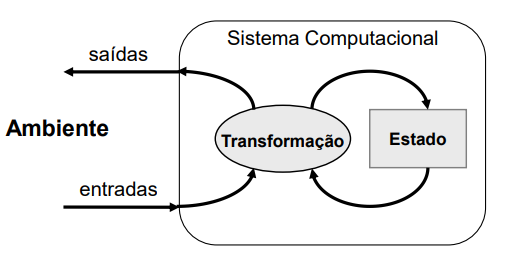
\includegraphics{../figures/sistema-computacional-abstrato}}
    \end{center}
    \caption{Modelo abstrato de um sistema computacional.
    Retirado de~\cite{isel:iasa:slides:intro-eng-soft-parte-3}, slide 3.}\label{fig:sistema-computacional-abstrato}
\end{figure}

Os conceitos fundamentais de um sistema computacional são:

\begin{itemize}
    \item \textbf{Dinâmica}: Descreve os estados que um sistema pode assumir
    e a forma como eles evoluem ao longo do tempo,
    determinando o comportamento do sistema;
    \item \textbf{Comportamento}: Expressa a estrutura de controlo do sistema, que corresponde à forma como o sistema age (gera as
    saídas) perante a informação proveniente do
    exterior (entradas) e do seu estado interno;
\end{itemize}

\subsection{Modelo formal de computação}\label{subsec:modelo-formal-de-computacao}

A função de transformação, mencionada anteriormente, pode ser decomposta em duas funções distintas (ver tabela~\ref{tab:funcoes-transformacao}), em que \textbf{Q} representa o conjunto de estados possíveis do sistema (regularmente designado por espaço de estados), \textbf{$\Sigma$} representa o conjunto de entradas possíveis e \textbf{Z} representa o conjunto de saídas possíveis.

\begin{table}[H]
    \centering
    \caption{Funções de Transformação de um Sistema Computacional}
    \label{tab:funcoes-transformacao}
    \vspace{0.2cm}
    \begin{tabular}{|l|l|p{8cm}|}
        \hline
        \textbf{Designação}          & \textbf{Expressão}                     & \textbf{Descrição}                                                                       \\ \hline
        Função de Transição (\delta) & \delta : Q \times \Sigma \rightarrow Q & Define a relação entre o estado do sistema e as entradas que recebe, e o próximo estado. \\ \hline
        Função de Saída (\lambda) & \lambda : Q \times \Sigma \rightarrow Z
        & Define a relação entre o estado do sistema e as entradas que recebe, e a saídas que produz. \\ \hline
    \end{tabular}
\end{table}

\begin{figure}[H]
    \begin{center}
        \resizebox{100mm}{!}{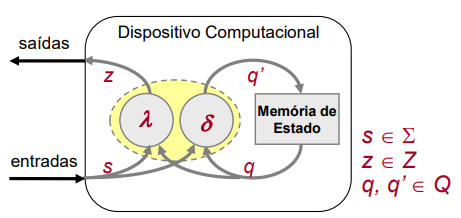
\includegraphics{../figures/modelo-sistema-computacional}}
    \end{center}
    \caption{Modelo de um sistema computacional.
    Retirado de~\cite{isel:iasa:slides:intro-eng-soft-parte-3}, slide 3.}\label{fig:modelo-sistema-computacional}
\end{figure}

Associado a um determinado modelo de um sistema computacional, está uma máquina de estados, que representa, de forma abstrata, o comportamento do sistema em função do tempo. Pode ser caracterizada por:

\begin{itemize}
    \item \textbf{Estado}: Se o número de estados possíveis é finito, então a máquina de estados é finita; caso contrário, é infinita;
    \item \textbf{Determinismo}: Uma máquina de estados finita também pode ser subcaracterizada em determinística (existe apenas uma transição para o mesmo estado e entrada) ou não determinística (existe mais do que uma transição para o mesmo estado e entrada).
    Para qualquer máquina de estados não determinística, existe uma máquina de estados determinística equivalente; \cite{wiki:finite-state-machine,freecodecamp:state-machines}
    \item \textbf{Função de Saída}: Se a função de saída $\lambda$ depende das entradas $\Sigma$, então a máquina de estados é do tipo \textit{Mealy} ($\lambda : Q \times \Sigma \rightarrow Z$); caso contrário, é do tipo \textit{Moore} ($\lambda : Q \rightarrow Z$).
\end{itemize}


\section{Desenvolvimento do Jogo}\label{sec:desenvolvimento-do-jogo}

Tendo por base os conceitos anteriormente abordados, que consolidaram a aprendizagem inerente à implementação da biblioteca, foi desenvolvido um jogo. No seu processo de desenvolvimento, foi definido um conjunto de componentes que providenciam implementações concretas dos subsistemas expostos pela biblioteca, adaptados ao contexto específico do jogo:

\begin{itemize}
    \item \textbf{Personagem}: Representa o agente do jogo;
    \item \textbf{Ambiente}: Representa o ambiente onde a Personagem opera;
    \item \textbf{Máquina de Estados}: Representa a máquina de estados associada ao controlo da Personagem.
    Caracterizada por ser finita, não determinística e do tipo \textit{Mealy} (Ver figura~\ref{fig:projeto-parte1-maqest-personagem}).
\end{itemize}

\begin{figure}[H]
    \begin{center}
        \resizebox{100mm}{!}{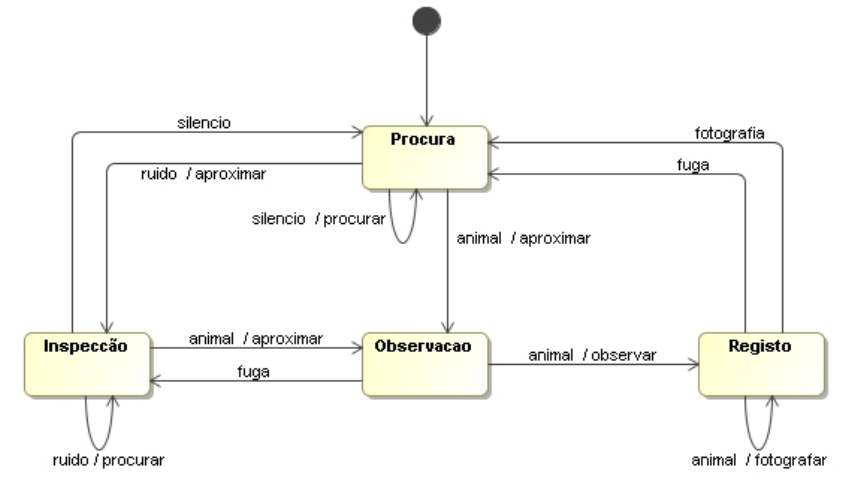
\includegraphics{../figures/projeto-parte1-maqest-personagem}}
    \end{center}
    \caption{Máquina de estados associada ao controlo da Personagem.
    Retirado de~\cite{isel:iasa:slides:intro-eng-soft-parte-3}, slide 14.}\label{fig:projeto-parte1-maqest-personagem}
\end{figure}

O jogo consiste num ambiente virtual onde a personagem tem por objectivo registar a presença de animais através de fotografias, simulando a exploração no mundo real.
Pode ser caracterizado (ver secção~\ref{sec:ambiente}) por ser:

\begin{itemize}
    \item \textbf{Parcialmente observável}: A Personagem apenas sabe o que está no seu campo de visão, e por isso precisa de explorar o ambiente para descobrir o que está à sua volta, necessitando de guardar estado interno para tomar decisões (e.g., se observou um animal anteriormente, então pode registar a sua presença);
    \item \textbf{Agente único}: Considerou-se que a Personagem é a única a atuar no ambiente no contexto do problema, visto que os animais são tratados como objetos passivos e integrantes do ambiente;
    \item \textbf{Estocástico}: Porque o estado seguinte pode depender de eventos aleatórios (e.g., a fuga de um animal) e não somente do estado atual e da ação da Personagem;
    \item \textbf{Sequencial}: Pois existe uma linha de acontecimentos que se sucedem (e.g., não é possível inspecionar, registar ou observar algo sem ser feita primeiro uma procura);
    \item \textbf{Dinâmico}: Pois o ambiente pode mudar enquanto a Personagem está a tomar uma decisão (e.g., os animais podem fugir);
    \item \textbf{Discreto}: Pois o número de estados possíveis é finito (e.g., pode ser mapeado para uma máquina de estados finita).
\end{itemize}

Foi criada uma aplicação (ver figura~\ref{fig:projeto-parte1-jogo}) de \textif{cli} (i.e., command-line interface) em Java, que possibilita a interação com o jogador por meio de comandos em texto.
Tendo em conta que a interface gráfica não era o foco desta parte do projeto, foi emulada através de texto descritivo.

\begin{figure}[H]
    \begin{center}
        \resizebox{100mm}{!}{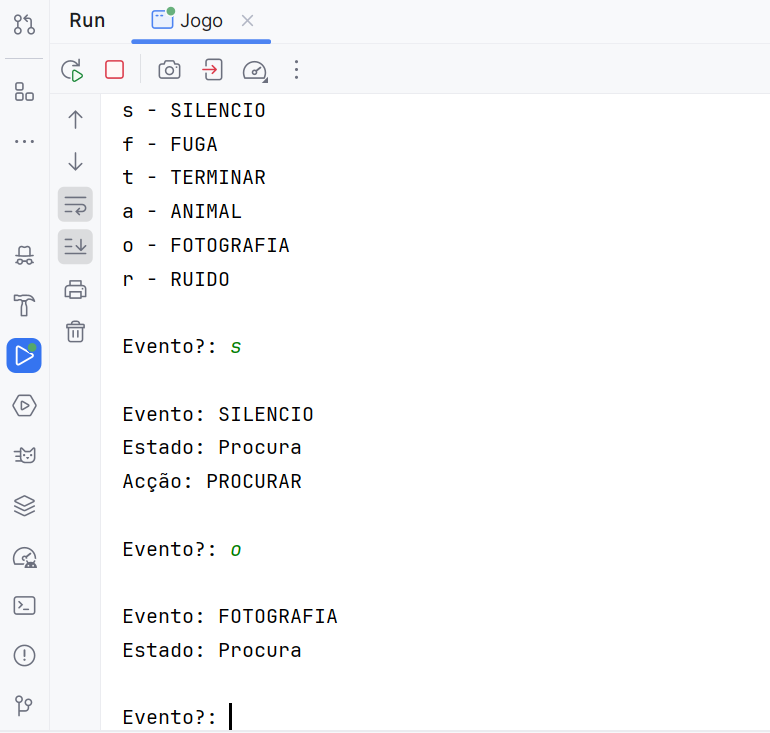
\includegraphics{../figures/projeto-parte1-jogo}}
    \end{center}
    \caption{Utilização da aplicação do jogo.}\label{fig:projeto-parte1-jogo}
\end{figure}


\section{Estrutura do Projeto}\label{sec:estrutura-do-projeto}

No processo de desenvolvimento de software associado a esta fase do projeto, foi definida a seguinte estrutura em módulos e que está presente na pasta \ti{iasa\_jogo/src}:

\begin{itemize}
    \item \textit{agente}: Integra classes e interfaces que definem o Agente e os seus componentes (e.g., módulo de controlo);
    \item \textit{ambiente}: Agrega interfaces que representam o Ambiente e os seus componentes (e.g., comandos, eventos);
    \item \textit{maqest}: Contém classes que definem o conceito de Máquina de Estados e os seus componentes (e.g., estados, transições);
    \item \textit{jogo}: Agrega os detalhes da implementação do jogo, onde são integrados os módulos anteriores e definidas implementações concretas dos mesmos, adequadas ao contexto a que o jogo se insere.
\end{itemize}
